\section{Results}
\label{sec:eval}

\subsection{Input Graph Characteristics}

We selected eleven graphs to analyze. Although we originally chose several 
others, we were limited by the hardware we had the funds to rent to analyzing 
relatively small graphs. A tradeoff exists between the size of a graph, the 
number of workers assigned to handle its vertices, and the amount of memory on 
a server. First, there is a minimum amount of memory that a Giraph worker 
requires in 
order to run. This puts an upper bound on the number of workers that can be run 
on any machine. Second, there appears to be a minimum number of workers that 
can be assigned to a graph of a given size in Giraph: when too few are 
assigned, the job fails. Presumably, this is because each worker can only 
feasibly handle a certain number of vertices, although it is unclear why Giraph 
chooses to terminate jobs rather than allowing them to eventually complete. 
This factor puts a lower bound on the number of workers that can be assigned to 
a graph, which is dependent on the size of the graph. Given these constraints, 
we restricted ourselves to graphs with approximately 200 million edges or fewer.

Our graphs came from 

We also paid attention to the distribution of the degrees of the vertices in 
the graphs that we chose. Since most natural graphs are power-law distributed, 
our graphs primarily follow that pattern. Figure \ref{fig:degree_distribution} 
shows a representative example of the degree distribution of a graph in our 
dataset.  (specifically, an imitation of Facebook's social graph, with 50 
million 
edges)

\begin{figure}
	\centering
	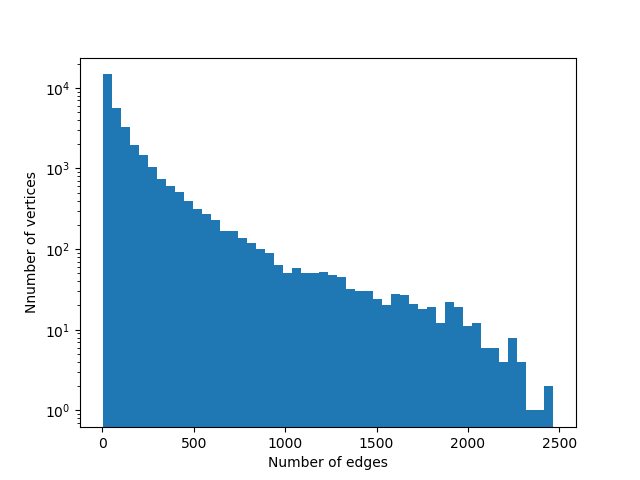
\includegraphics[width=\columnwidth]{../good_plots/degree_distribution_10_mil.png}
	\caption{Degree distribution for a representative graph in our dataset, 
	demonstrating that the graphs we chose are power-law graphs.}
	\label{fig:degree_distribution}
\end{figure}

\begin{figure}
	\centering
	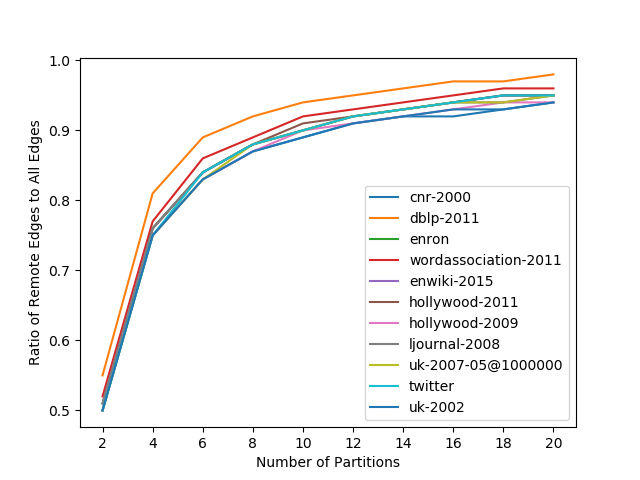
\includegraphics[width=\columnwidth]{../good_plots/remote_to_all_modulo.png}
	\caption{Ratio of remote edges (requiring messages to be sent across the 
	network) to all edges for various numbers of partitions, where partitioning 
	is done by taking the modulus of the vertex ID and number of workers.}
	\label{fig:remote_to_all_mod}
\end{figure}

\begin{figure}
	\centering
	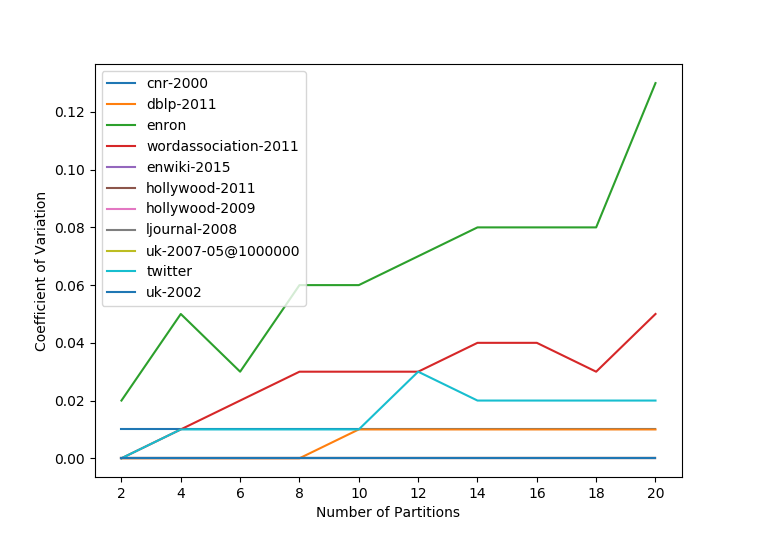
\includegraphics[width=\columnwidth]{../good_plots/range_as_cv_modulo.png}
	\caption{Range of the maximum number of edges handled by each worker to the 
	minimum handled by any worker, expressed by the coefficient of variation, 
	for various numbers of partitions, with modulo partitioning.}
	\label{fig:cv_mod}
\end{figure}

\begin{figure}
	\centering
	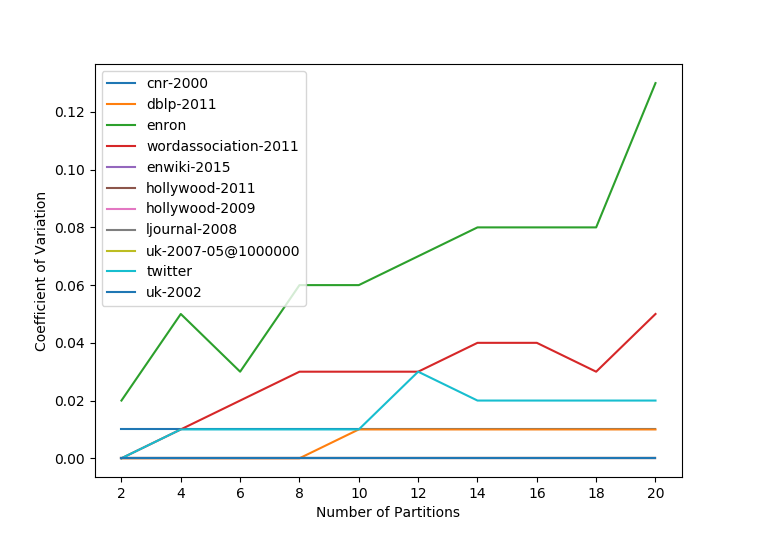
\includegraphics[width=\columnwidth]{../good_plots/range_as_cv_modulo.png}
	\caption{Range of the maximum number of edges handled by each worker to the 
		minimum handled by any worker, expressed by the coefficient of 
		variation, for various numbers of partitions, with segmented 
		partitioning.}
	\label{fig:cv_range}
\end{figure}

\begin{figure}
	\centering
	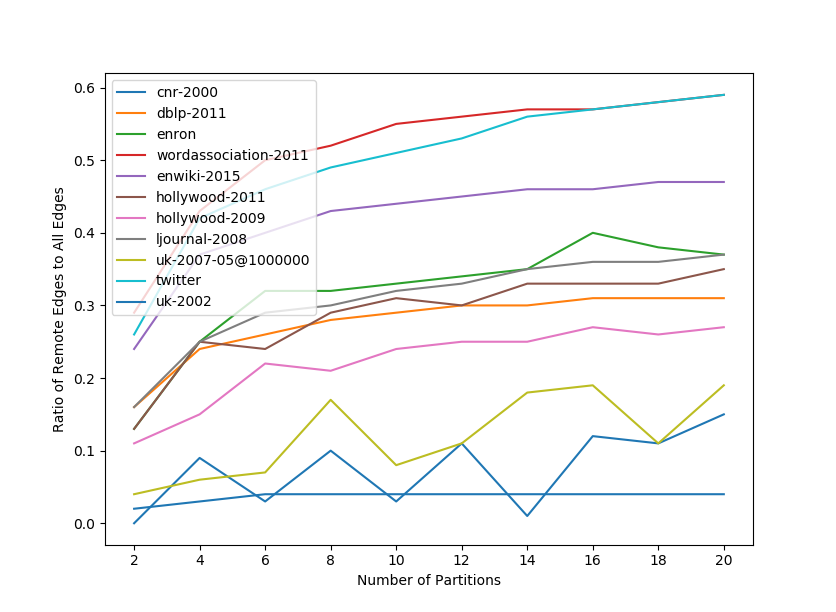
\includegraphics[width=\columnwidth]{../good_plots/remote_to_all_chunked.png}
	\caption{Ratio of remote edges to all edges for various numbers of 
	partitions, where partitioning is done by segmenting the vertex IDs into 
	approximately equal groups.}
	\label{fig:remote_to_all_range}
\end{figure}

\subsection{Setting up Giraph}
1. Look at all the settings file and decribe important settings 
2. JNI error due to Java version mismatch
3. Lot of effort spent in adjusting getting the resource limits right
    - too many files to set configurations
    - no facilities for fine-tuned resource allocation - lot of out of memory exceptions due to tuning errors
    - incomprehensible error messages or errors hidden in remote corners of unknown log files
    - super-fragile, one change in setting causes an error in a completely unrelated place.
    - 8 hours from getting giraph built to getting the first job running without excepts
4. 

\subsection{Effect of different partition schemes}
